\chapter{弗里德曼动力学：物质、辐射与真空能}

\lectureoverview{膨胀宇宙的运动学可以用一句话表述：物理间距随标度因子\(a(t)\)增长。现在的问题是要确定这个函数。我们将从牛顿能量守恒重新导出平直空间的弗里德曼方程，先对普通物质求解，然后看看为什么辐射和真空能会导致完全不同的宇宙历史。}

\section{待解释的几何}

在固定的宇宙时刻，大尺度宇宙看起来是均匀且各向同性的。星系、星系团和超星系团当然是真实的结构，但在数亿或数十亿光年的尺度上，它们的分布变得非常均匀。这一经验规律被称为宇宙学原理。这个名称并不能使它成为一条定理；该原理的力量来自观测。

还有第二个经验事实。在目前的精度范围内，大的空间三角形表现得如同欧几里得三角形。与测量足球场的类比是有用的。如果拉紧的线构成的三角形的内角和为\(180^\circ\)，这并没有证明地球整体上是平的。它表明的是地球的曲率半径远大于足球场。宇宙测量具有相同的逻辑形式：空间可能具有非常大的曲率半径，但在可观测区域内，它可以很好地近似为平直的。

参考几何是闵可夫斯基时空，
\begin{equation}
  d\tau^2=dt^2-\left(dx^2+dy^2+dz^2\right).
  \label{eq:l09-minkowski}
\end{equation}
括号内就是三维的欧几里得距离元。相比之下，在广义相对论中，坐标微分的系数是场。它们可以随位置和时间变化，也可能出现混合项。这些度规系数是牛顿引力场的相对论后继者。

\begin{figure}[H]
  \centering
  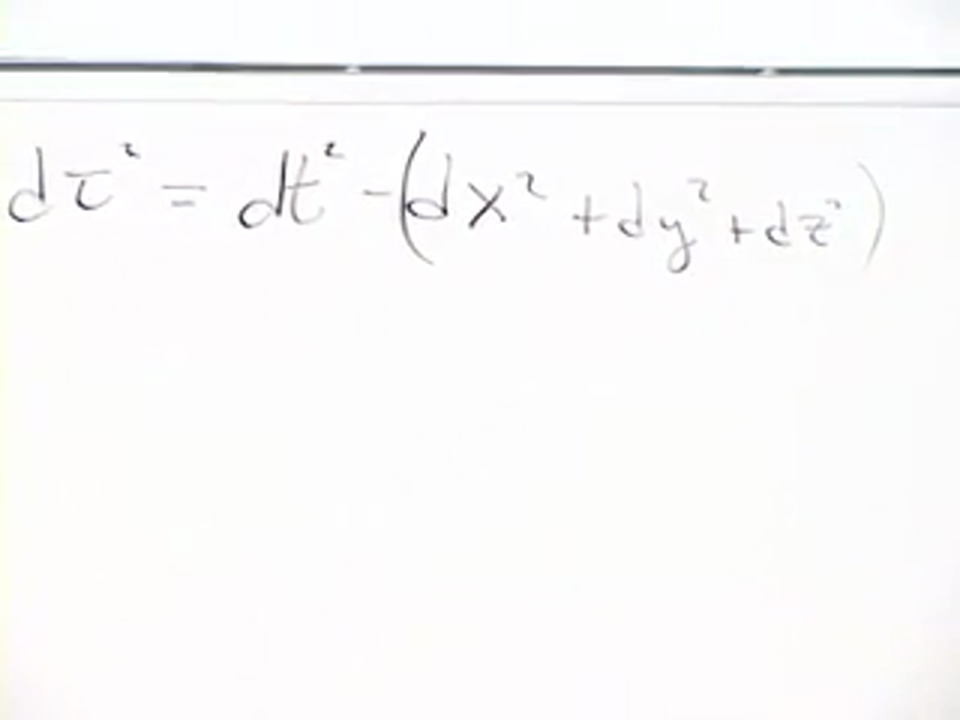
\includegraphics[width=0.72\textwidth]{lecture_09_figure_01.png}
  \caption{讲座开头写出的闵可夫斯基固有时元。源帧位于00:01:50。}
  \label{fig:l09-minkowski-board}
\end{figure}

对于空间平直的膨胀宇宙，均匀性和各向同性只留下一个依赖于时间的标度因子：
\begin{equation}
  d\tau^2=dt^2-a^2(t)\left(dx^2+dy^2+dz^2\right).
  \label{eq:l09-flat-frw}
\end{equation}
我们采用\(c=1\)的单位制，因此时间和长度具有相同的量纲。有两种自洽的约定。可以赋予\(x,y,z\)长度的量纲并取\(a\)无量纲，或者把\(x,y,z\)视为无量纲的标签而让\(a\)带有长度的量纲。本讲座采用第二种约定，因为它使\(a(t)\)的物理意义变得可见。

\begin{figure}[H]
  \centering
  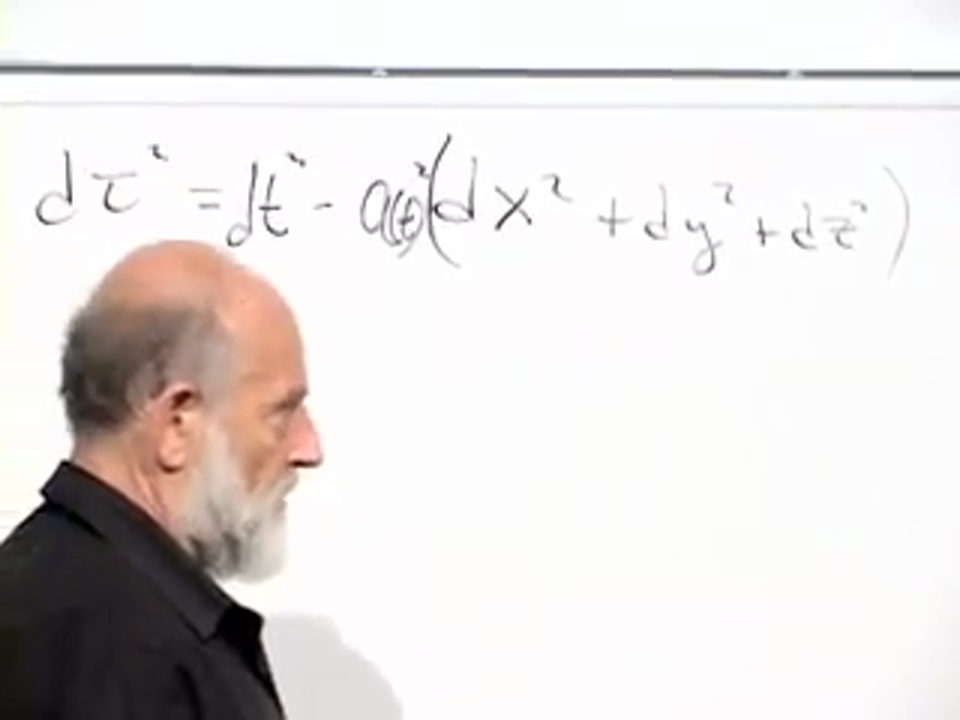
\includegraphics[width=0.72\textwidth]{lecture_09_figure_02.png}
  \caption{平直膨胀度规，其中标度因子乘以欧几里得空间线元。源帧位于00:09:12。}
  \label{fig:l09-expanding-metric-board}
\end{figure}

想象坐标被画在一块橡胶片上。坐标标记始终附着在橡胶片上，而它们之间的物理距离却在增长。因此，诸如“从\(x=0\)到\(x=1\)”这样的坐标差只是一对标签。该间隔所代表的距离是\(a(t)\)。找出支配这个标度因子的方程，就是本讲座的动力学问题。

\section{闭合、平直与开放的空间几何}

平直性是一种观测上的简化，而不是均匀性的结果。存在三种均匀且各向同性的空间几何：正曲率、零曲率和负曲率。要理解正曲率的情形，有必要对维数保持精确。

轨迹
\begin{equation}
  X_1^2+X_2^2=R^2
\end{equation}
是一个圆，即一维球面\(S^1\)。它填充的内部是一个圆盘，也称为二维球。增加一个嵌入坐标得到
\begin{equation}
  X_1^2+X_2^2+X_3^2=R^2,
\end{equation}
普通的二维球面\(S^2\)。再增加第四个嵌入坐标得到
\begin{equation}
  X_1^2+X_2^2+X_3^2+X_4^2=R^2,
  \label{eq:l09-three-sphere}
\end{equation}
三维球面\(S^3\)，它本身就是一个三维空间。我们无法想象它的四维嵌入，但内禀几何并不需要那个嵌入才能存在。

\begin{figure}[H]
  \centering
  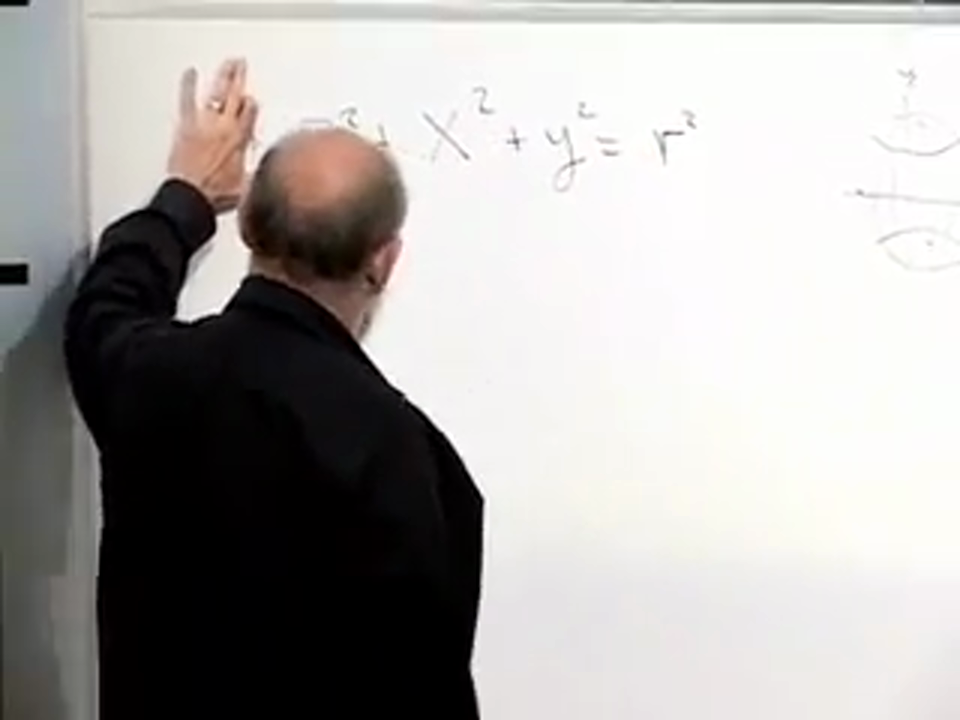
\includegraphics[width=0.72\textwidth]{lecture_09_figure_03.png}
  \caption{用于引入三维球面的嵌入方程。源帧位于00:16:40。}
  \label{fig:l09-three-sphere-board}
\end{figure}

理想球面上的每一点在几何上都与其他任何一点等价，一点处的每个方向也都等价。因此球面既是均匀的又是各向同性的。如果它的半径乘以\(a(t)\)，整个空间就会膨胀或收缩，而不会在球面上选出一个中心。将这样的宇宙回溯过去，并不会把所有物质都置于外部虚空中的一个特殊位置。整个空间都变小了，因此每一对点都彼此靠近。大爆炸并不是从空间中的某一点发生的爆炸。

在正曲率的球面上，测地三角形的内角和大于
\(180^\circ\)。平坦三角形的内角和恰好为 \(180^\circ\)。在由马鞍面不完美地代表的均匀负曲率几何中，内角和小于 \(180^\circ\)。这些内禀检验区分了这三种情形。

\begin{figure}[H]
  \centering
  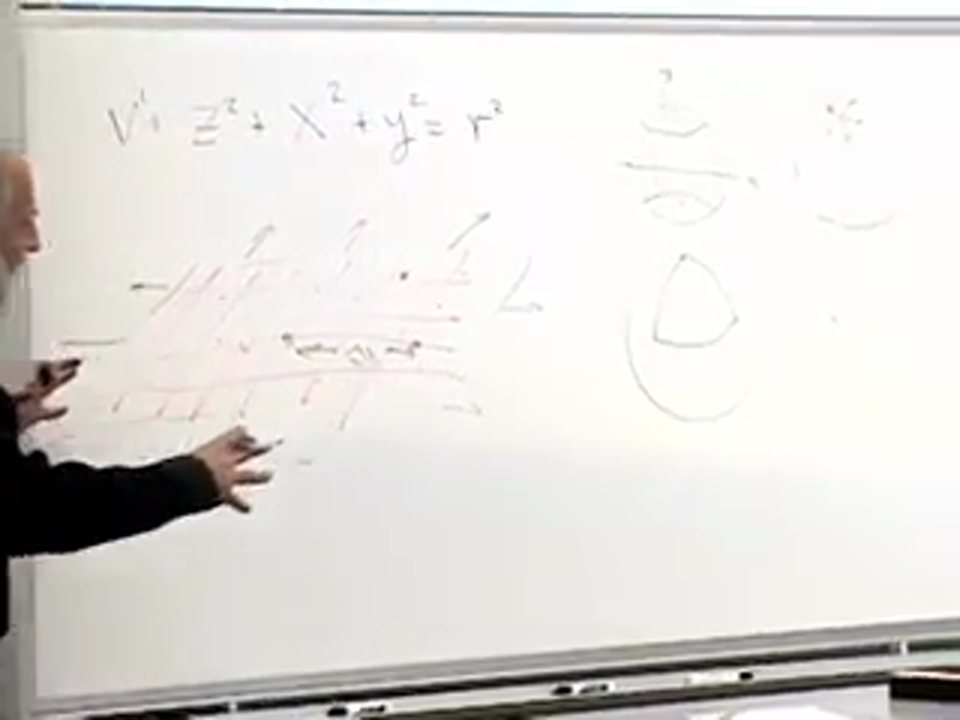
\includegraphics[width=0.72\textwidth]{lecture_09_figure_07.png}
  \caption{通过其特征三角形形状勾勒出的正、零与负曲率。源帧位于 00:37:30。}
  \label{fig:l09-curvature-board}
\end{figure}

一个完全平坦的局部度规本身并不能证明空间在拓扑上是无限的。紧致平坦拓扑在数学上是可能的，尽管本讲采用最简单的无限欧几里得模型。
\editorialnote{这一整体拓扑上的限定条件对于后续任何局部动力学都不需要。}

\section{共动标签与哈勃定律}

现在回到膨胀的平坦薄片，并在其上画一个坐标网格。在共动坐标中，网格随大尺度物质流一起膨胀。一个星系，或者更准确地说，一个足够粗粒化的星系团，保持近似固定的坐标标签，尽管它与另一个共动物体的物理距离在变化。

\begin{figure}[H]
  \centering
  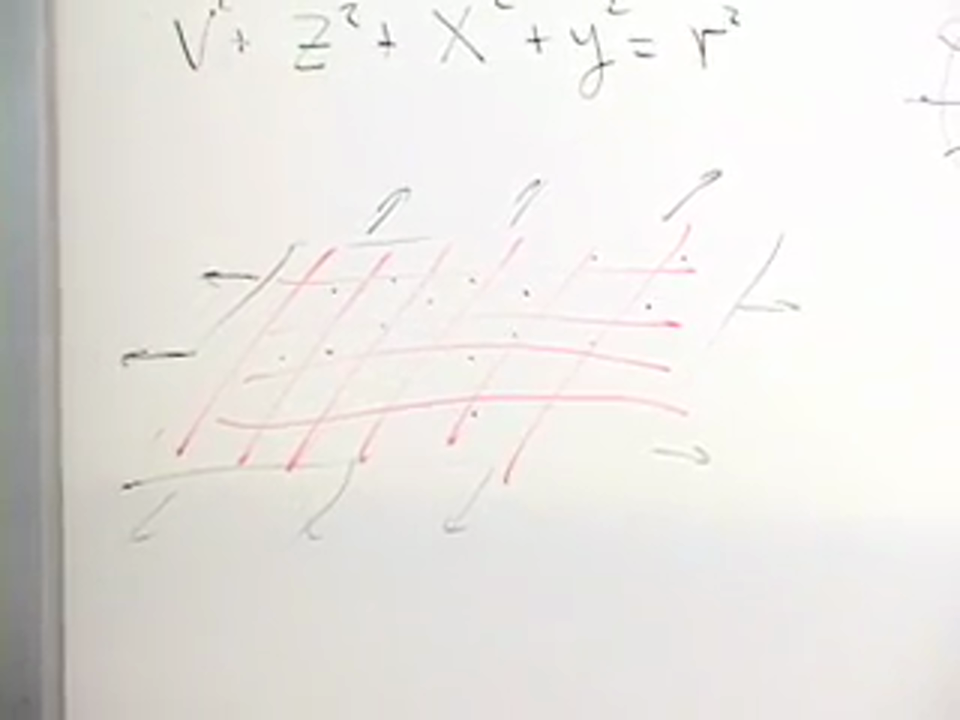
\includegraphics[width=0.72\textwidth]{lecture_09_figure_04.png}
  \caption{随膨胀空间薄片一起被携带的坐标网格。
  源帧位于 00:22:20。}
  \label{fig:l09-comoving-grid-board}
\end{figure}

对于沿 \(x\) 轴以固定共动间隔 \(\Delta x\) 分隔的两个物体，它们的物理距离为
\begin{equation}
  D(t)=a(t)\,\Delta x.
  \label{eq:l09-physical-distance}
\end{equation}
在保持 \(\Delta x\) 固定的情况下求导，得到
\begin{equation}
  v(t)=\dot a(t)\,\Delta x
      =\frac{\dot a(t)}{a(t)}D(t).
\end{equation}
定义
\begin{equation}
  H(t)\equiv\frac{\dot a(t)}{a(t)},
  \label{eq:l09-hubble-parameter}
\end{equation}
我们得到哈勃定律，
\begin{equation}
  v=H(t)D.
  \label{eq:l09-hubble-law}
\end{equation}
“哈勃常数”中的“常数”一词意味着在指定的宇宙时刻在空间各处为常数。它并不意味着在整个宇宙历史中恒定不变。

\begin{figure}[H]
  \centering
  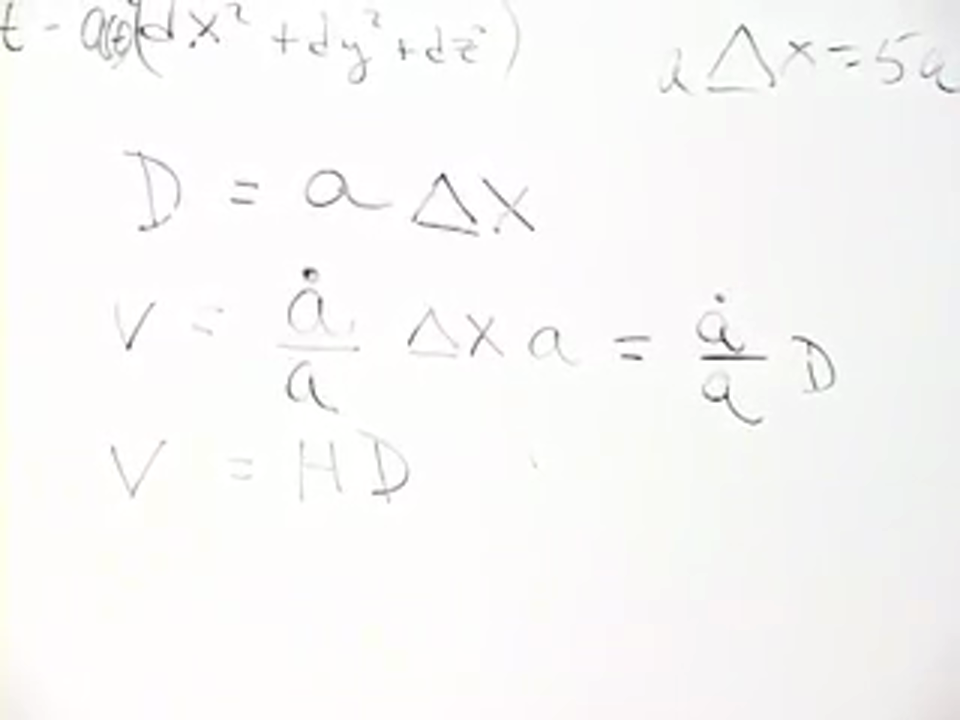
\includegraphics[width=0.72\textwidth]{lecture_09_figure_05.png}
  \caption{黑板推导 \(D=a\Delta x\)，
  \(v=(\dot a/a)D=HD\)。源帧位于 00:26:40。}
  \label{fig:l09-hubble-board}
\end{figure}

\begin{classroomqa}
\audiencequestion{如果一个遥远星系是在更早的时刻被看到的，那么推断出的哈勃参数真的应该等于今天在附近测得的值吗？}
\lecturerresponse{只有当回溯时间与宇宙年龄相比很小时才是如此。在中等距离上，\(H(t)\) 变化足够小，以至于一个数值仍然有用。在真正宇宙学尺度上，我们看到的是更早的时期，因此必须计入 \(a\) 和 \(H\) 的时间依赖性。这就是我们需要关于标度因子的动力学方程的原因之一。}
\end{classroomqa}

\section{膨胀坐标系中的零测地线}

\begin{classroomqa}
\audiencequestion{标度因子会影响光在遥远星系之间的传播吗？}
\lecturerresponse{光线沿零测地线传播，因此 \(d\tau=0\)。对于沿正 \(x\) 轴运动的光线，\(dy=dz=0\)，而膨胀的度规给出
\begin{align}
  0&=dt^2-a^2(t)dx^2,
  &dt&=a(t)dx,\notag\\
  &&\frac{dx}{dt}&=\frac{1}{a(t)}.
  \label{eq:l09-null-ray}
\end{align}
坐标速度随着 \(a(t)\) 增大而减小，但光的局部物理速度仍为 \(c=1\)。固定的坐标间隔代表不断增大的物理距离。}
\end{classroomqa}

\begin{figure}[H]
  \centering
  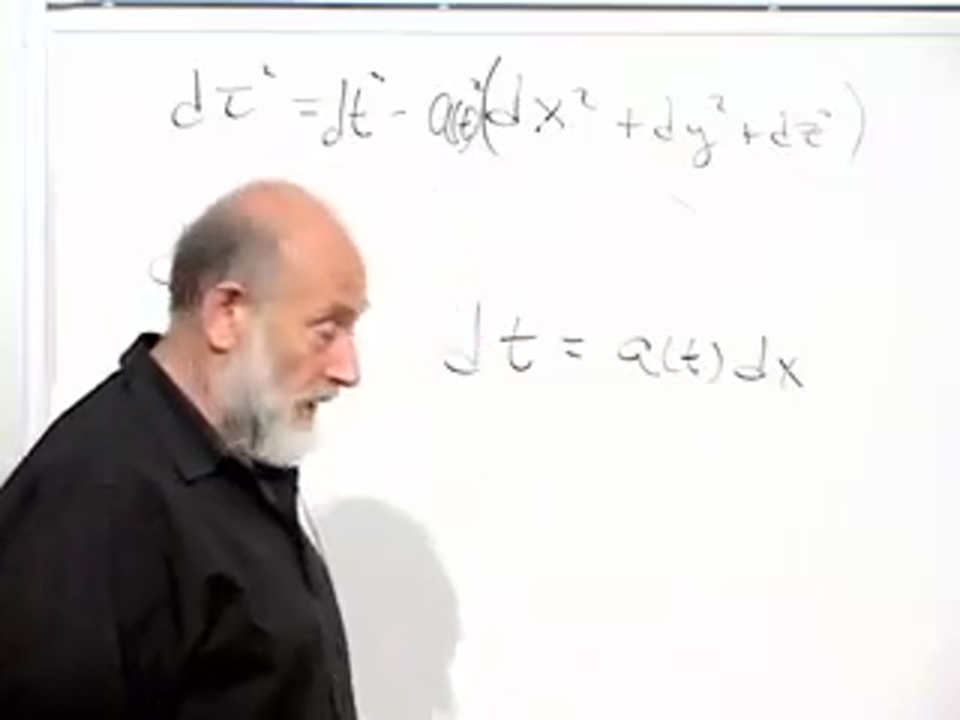
\includegraphics[width=0.72\textwidth]{lecture_09_figure_06.png}
  \caption{零条件与径向光传播的 \(dt=a(t)dx\)。
  源帧位于 00:30:54。}
  \label{fig:l09-null-board}
\end{figure}

人们可以选择这样的坐标，使得同一事实听起来像是“光在更远处变慢”，但这样一来，长度和时钟就会获得相应别扭的描述。膨胀空间的语言更简洁，因为它保留了局部陈述：每个自由下落的观测者测得相同的光速。

\begin{classroomqa}
\audiencequestion{有证据表明遥远星系中的局部光传播和原子物理是相同的吗？}
\lecturerresponse{只有无量纲比较在操作上才有意义。选择原子尺度作为长度单位，选择原子或核周期作为时间单位，然后问光穿过所选长度需要多少个这样的周期。光谱观测支持这样的陈述：这些无量纲比值在遥远区域是相同的。证据是间接的，但它恰恰是用来检验局部定律均匀性的那类比较。}
\end{classroomqa}

当可观测宇宙极其小时，光可以在相应的光穿越单位内迅速穿过给定的物理区域。这并不意味着 \(c\) 不同。它意味着该区域本身很小。

\section{宇宙内部的牛顿球}

现在我们从运动学转向动力学。把我们自己置于原点，画一个足够大的球面，使其包含许多星系和星系团。在其边界上选取一个星系。在均匀宇宙中，质量分布相对于我们呈球对称，而牛顿壳层定理给出两个关键事实：
\begin{enumerate}
  \item 所有分布在所选半径之外的球对称物质，对边界星系施加的净牛顿力为零；
  \item 球内所有物质，对于这种径向运动而言，其作用就如同全部集中在中心一样。
\end{enumerate}
我们使用一个我们处于静止的参考系，因此以下论证中的速度和加速度都是相对于我们测量的。

\begin{figure}[H]
  \centering
  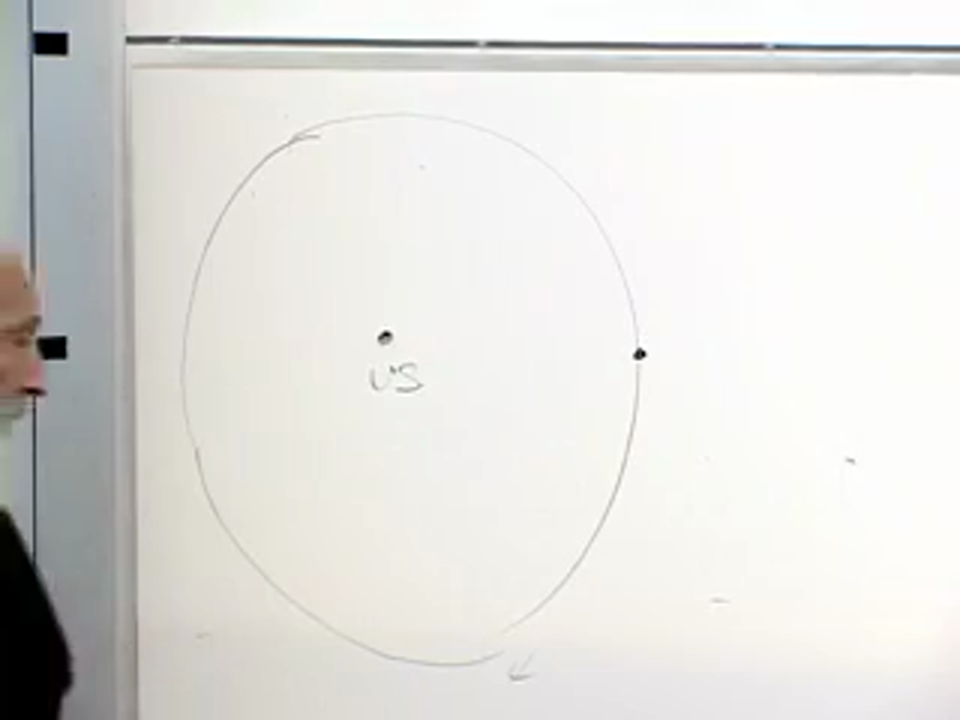
\includegraphics[width=0.72\textwidth]{lecture_09_figure_08.png}
  \caption{壳层定理的构造：我们位于中心，一个测试星系位于一个大的均匀球面的边界上。源帧位于 00:41:10。}
  \label{fig:l09-shell-board}
\end{figure}

\begin{figure}[H]
  \centering
  \begin{tikzpicture}[scale=0.92,>=Latex]
    \draw[thick] (0,0) circle (2.35);
    \fill (0,0) circle (2pt) node[below left] {us};
    \fill (2.35,0) circle (2.2pt) node[right] {test galaxy \(m\)};
    \draw[->,thick,blue!65!black] (0.18,0) -- (2.15,0)
      node[midway,above] {\(R=a(t)x\)};
    \draw[->,thick,red!65!black] (2.35,0.12) -- (3.25,0.12)
      node[midway,above] {\(v=\dot a(t)x\)};
    \node[align=center,text width=7cm] at (0,-2.85)
      {outside shells cancel;\\enclosed mass acts at the center};
  \end{tikzpicture}
  \caption{牛顿构造的清晰重建。}
  \label{fig:l09-shell-clean}
\end{figure}

如果该星系具有固定的共动坐标 \(x\)，则其物理半径和速度为
\begin{equation}
  R(t)=x a(t),
  \qquad
  v(t)=x\dot a(t)=H(t)R(t).
  \label{eq:l09-radius-velocity}
\end{equation}
设 \(M\) 为球面所包围的质量，\(m\) 为测试星系的质量。牛顿能量为
\begin{equation}
  E=\frac12 m v^2-\frac{GMm}{R}.
  \label{eq:l09-newtonian-energy}
\end{equation}

\begin{figure}[H]
  \centering
  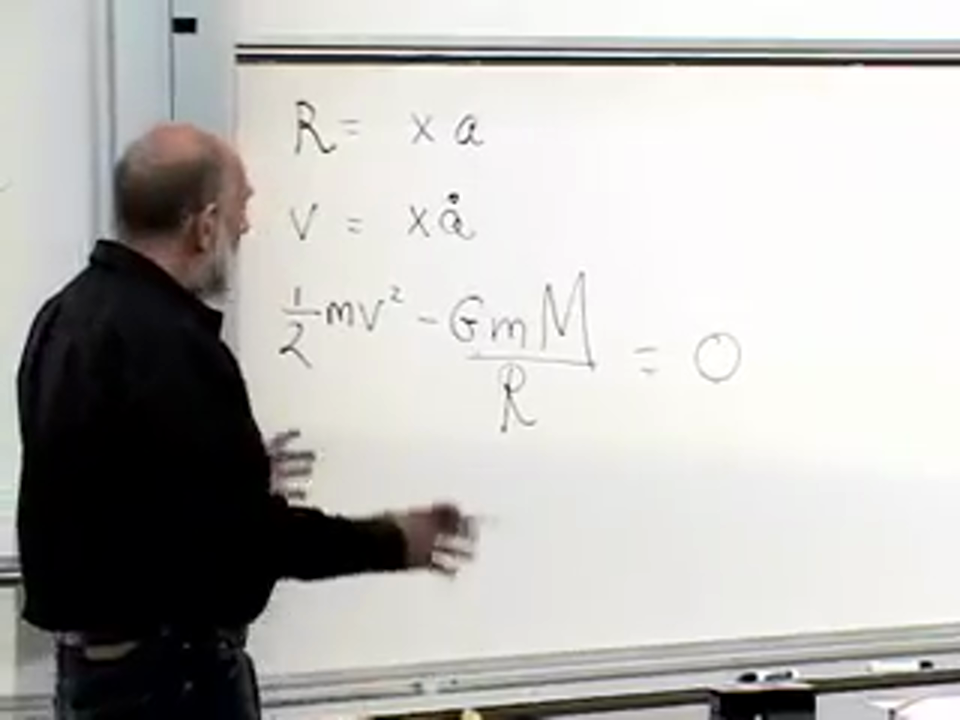
\includegraphics[width=0.72\textwidth]{lecture_09_figure_09.png}
  \caption{完整的板书序列 \(R=xa\)、\(v=x\dot a\)，以及针对 \(E=0\) 特化的牛顿能量方程。源帧位于 00:48:40。}
  \label{fig:l09-energy-board}
\end{figure}

能量可以为正、为零或为负。从逃逸与再坍缩之间的边界开始，\(E=0\)，对此有
\begin{equation}
  \frac12 v^2=\frac{GM}{R}.
  \label{eq:l09-zero-energy}
\end{equation}

\begin{classroomqa}
\audiencequestion{对于退行星系，总能量为零意味着什么？}
\lecturerresponse{这恰好就是逃逸速度的情形。正的能量意味着运动高于逃逸速度；负的能量意味着运动低于逃逸速度，并且在仅有物质的牛顿图像中，最终会返回。我们从这些可能性之间的边界开始，并在推导出平坦方程之后再回到其他符号。}
\end{classroomqa}

\begin{classroomqa}
\audiencequestion{所包围的质量 \(M\) 会随着球面膨胀而变化吗？}
\lecturerresponse{不会。该球面是共动的，因此同样的粒子始终留在其内部。它的物理体积增大，密度下降，但其总包围质量保持固定。\(M\) 与 \(\rho(t)\) 之间的这一区分至关重要。}
\end{classroomqa}

对于均匀密度 \(\rho(t)\)，
\begin{equation}
  M=\frac{4\pi}{3}\rho(t)R^3.
  \label{eq:l09-enclosed-mass}
\end{equation}
代入 \eqref{eq:l09-zero-energy} 得到
\begin{equation}
  \frac12 v^2
  =\frac{G}{R}\left(\frac{4\pi}{3}\rho R^3\right).
  \label{eq:l09-enclosed-energy}
\end{equation}

\begin{figure}[H]
  \centering
  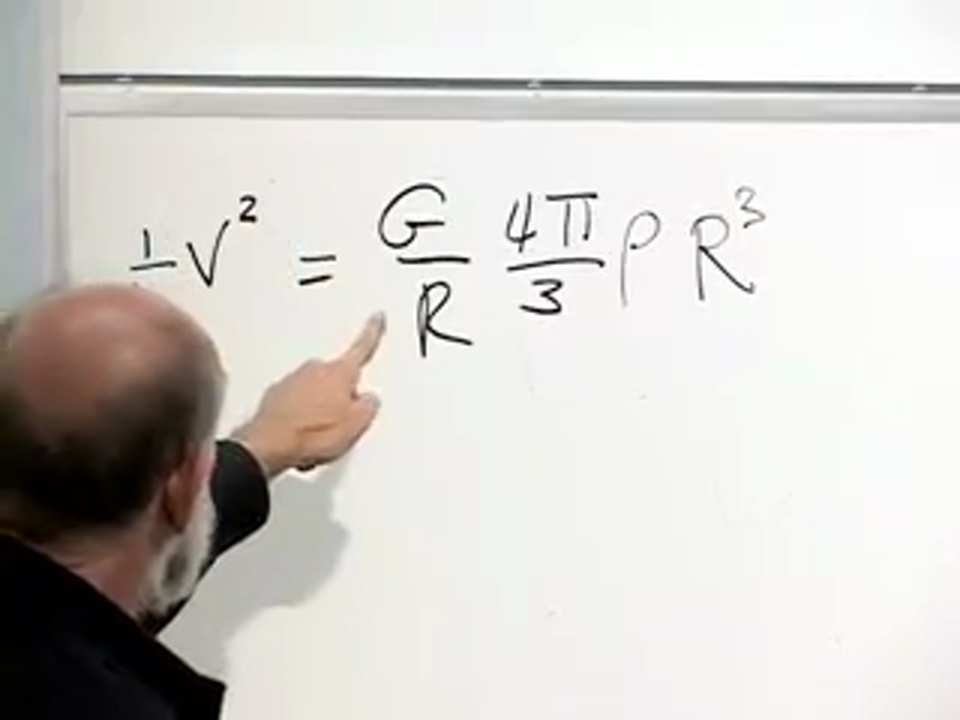
\includegraphics[width=0.72\textwidth]{lecture_09_figure_10.png}
  \caption{零能量方程中的包围质量代换。源帧位于 00:54:16.060。}
  \label{fig:l09-enclosed-mass-board}
\end{figure}

利用 \(v=HR\)，我们得到
\begin{align}
  \frac12 H^2R^2
    &=\frac{4\pi G}{3}\rho R^2,\\
  H^2
    &=\frac{8\pi G}{3}\rho.
\end{align}
因此，零能量、空间平坦的膨胀定律为
\begin{equation}
  \boxed{\left(\frac{\dot a}{a}\right)^2
  =\frac{8\pi G}{3}\rho(t)}.
  \label{eq:l09-flat-friedmann}
\end{equation}
\(R^2\) 的消去并非偶然。一个均匀宇宙无论选择哪个共动星系作为测试对象，都必须给出相同的 \(H(t)\)。

\begin{figure}[H]
  \centering
  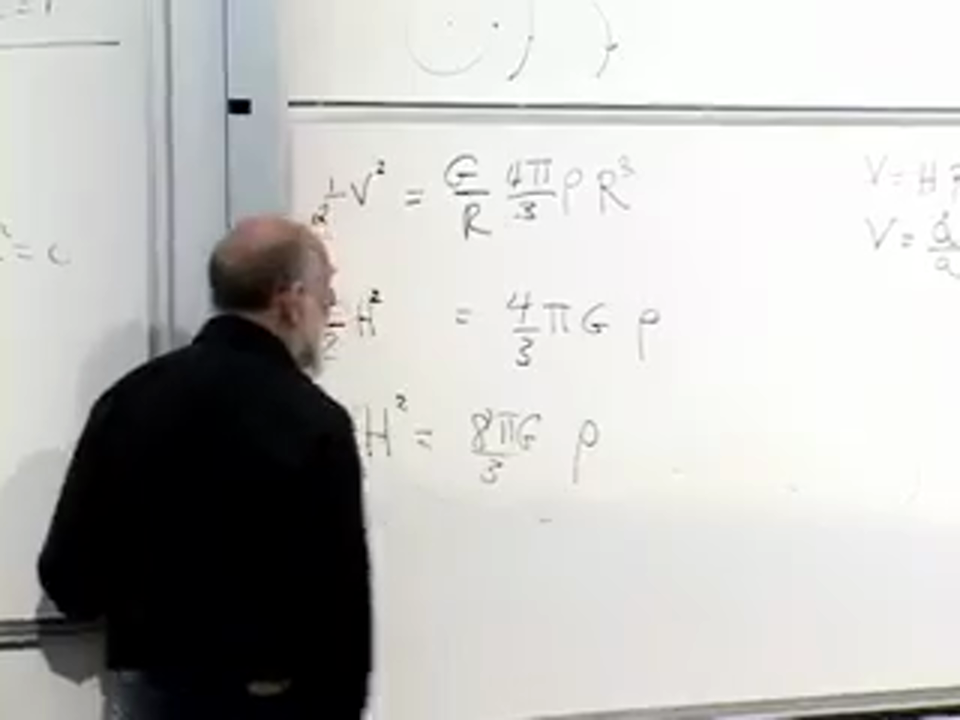
\includegraphics[width=0.72\textwidth]{lecture_09_figure_11.png}
  \caption{半径的消去以及由此得到的平坦弗里德曼关系在板书上。源帧位于 00:57:30。}
  \label{fig:l09-friedmann-board}
\end{figure}

\begin{classroomqa}
\audiencequestion{有证据支持零能量关系吗？}
\lecturerresponse{两边都可以通过观测推断：\(H\) 来自退行数据，而 \(\rho\) 则通过计入恒星、气体、暗物质和真空能量得到。讲座时代的比较发现两边在约百分之几的精度内一致。这一限定很重要：必须包括所有形式的能量，而后面对真空能量的讨论会改变朴素的逃逸速度解释。}
\end{classroomqa}

在单位 \(c=1\) 下，质量密度和能量密度具有相同的单位。因此符号 \(\rho\) 将表示适用于所讨论组分的总能量密度。

\section{普通物质与三分之二定律}

方程 \eqref{eq:l09-flat-friedmann} 在知道 \(\rho(t)\) 如何变化之前并不封闭。首先用一个缓慢运动的非相对论性粒子填充一个共动长方体盒子。它的坐标尺寸固定，而其物理体积按如下方式增长：
\begin{equation}
  V(t)=a^3(t)\,\Delta x\,\Delta y\,\Delta z.
\end{equation}
盒子中的粒子数和静质量保持固定，因此
\begin{equation}
  \rho_{\mathrm m}(t)=\frac{C_{\mathrm m}}{a^3(t)}.
  \label{eq:l09-matter-dilution}
\end{equation}
归一化到当前时期 \(t_0\)，
\begin{equation}
  \frac{\rho_{\mathrm m}(t)}{\rho_{\mathrm m,0}}
  =\left(\frac{a_0}{a(t)}\right)^3.
  \label{eq:l09-matter-normalized}
\end{equation}

\begin{figure}[H]
  \centering
  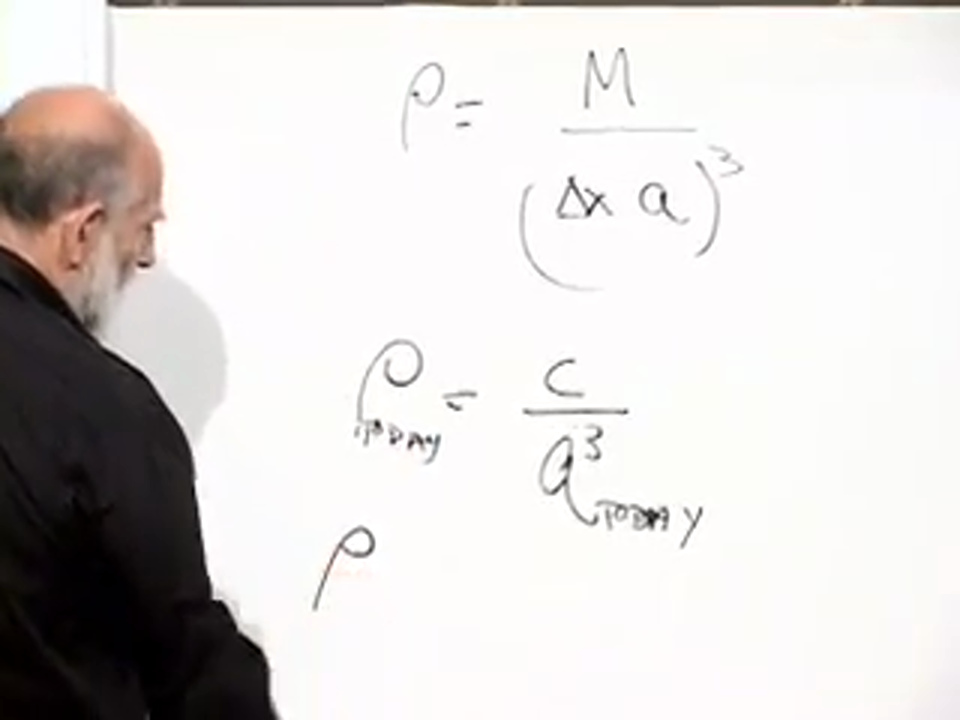
\includegraphics[width=0.72\textwidth]{lecture_09_figure_12.png}
  \caption{物质密度、其 \(a^{-3}\) 稀释以及当今归一化。源帧位于 01:04:47.940。}
  \label{fig:l09-density-board}
\end{figure}

\begin{classroomqa}
\audiencequestion{目前宇宙的能量密度大致是多少，仅靠普通原子能提供吗？}
\lecturerresponse{对可见重子物质的计数只给出了答案的一部分。暗物质和暗能量也必须以等效质能的形式计入。讲座引用了一个粗略的尺度范围，从每立方米一个原子到几十个氢质量当量，强调的是数量级而非精确清单。}
\end{classroomqa}

将\eqref{eq:l09-matter-dilution}代入\eqref{eq:l09-flat-friedmann}，并把所有与时间无关的因子吸收进一个正常数\(C\)：
\begin{equation}
  \left(\frac{\dot a}{a}\right)^2=\frac{C}{a^3},
  \qquad
  \dot a^2=\frac{C}{a}.
  \label{eq:l09-matter-ode}
\end{equation}
有两种直截了当的方法可以求解它。幂律试探解\(a=K t^p\)要求
\begin{equation}
  p-1=-\frac{p}{2},
  \qquad p=\frac23.
\end{equation}
等价地，取膨胀的平方根分支并积分：
\begin{equation}
  a^{1/2}\frac{da}{dt}=\sqrt C,
  \qquad
  \int a^{1/2}da=\sqrt C\int dt,
\end{equation}
因此，在选定大爆炸作为时间原点之后，
\begin{equation}
  a^{3/2}\propto t,
  \qquad
  \boxed{a(t)\propto t^{2/3}}.
  \label{eq:l09-matter-solution}
\end{equation}
现场推导在匹配系数时短暂丢失了一个因子，随后回到积分并验证了指数。笔记保留了这一检验，但只展示修正后的代数运算。

\begin{figure}[H]
  \centering
  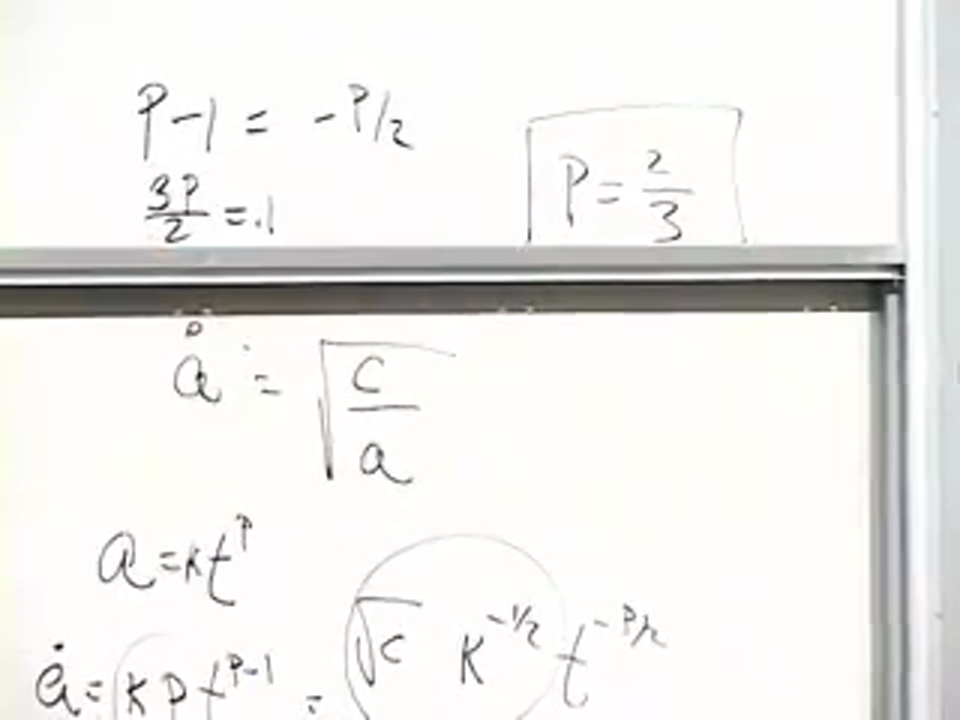
\includegraphics[width=0.72\textwidth]{lecture_09_figure_13.png}
  \caption{幂律试探解与加框的指数\(p=2/3\)。源帧位于01：13：05。}
  \label{fig:l09-matter-solution-board}
\end{figure}

对解求导得到
\begin{equation}
  H(t)=\frac{\dot a}{a}=\frac{2}{3t}.
  \label{eq:l09-matter-hubble}
\end{equation}
哈勃参数在过去更大。因此，当看得足够远以观察到可观的回溯时间时，不应使用今天的\(H_0\)不变来外推局域线性关系。

\begin{figure}[H]
  \centering
  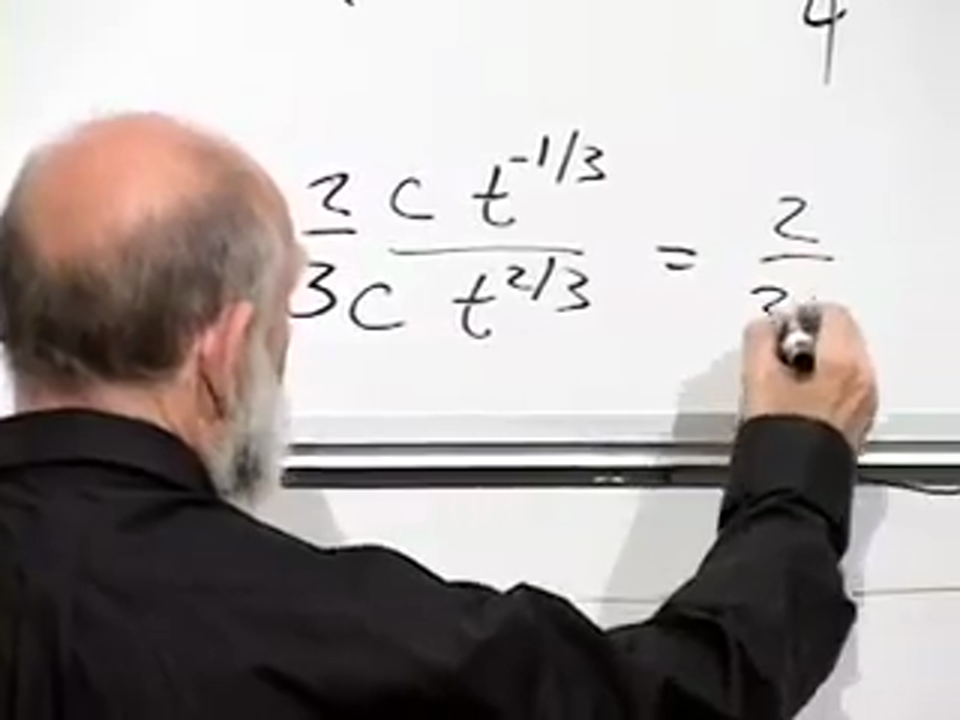
\includegraphics[width=0.72\textwidth]{lecture_09_figure_14.png}
  \caption{取\(\dot a/a\)对于\(a\propto t^{2/3}\)得到
  \(H=2/(3t)\)。源帧位于01：20：42。}
  \label{fig:l09-hubble-time-board}
\end{figure}

\section{能量符号与空间曲率}

牛顿式的推理已经带领我们走过了平坦的零能量情形。广义相对论补充了一个仅靠壳层定理无法得到的事实：牛顿式比能量的符号对应于空间曲率的符号。
\begin{center}
\begin{tabular}{@{}>{\raggedright\arraybackslash}p{0.20\linewidth}
                    >{\raggedright\arraybackslash}p{0.29\linewidth}
                    >{\raggedright\arraybackslash}p{0.37\linewidth}@{}}
  \toprule
  总能量 & 空间曲率 & 仅含物质时的命运 \\
  \midrule
  正 & 负（开放） & 永远膨胀 \\
  零 & 零（平坦） & 趋近逃逸边界 \\
  负 & 正（闭合） & 膨胀、反转、再坍缩 \\
  \bottomrule
\end{tabular}
\end{center}
最后一列假设没有真空能。在抛射体类比中，正能量意味着高于逃逸速度，零意味着恰好等于逃逸速度，负意味着低于逃逸速度。爱因斯坦方程将这三种情形分别与开放、平坦和闭合的空间几何对应起来。

\section{光子与二分之一定律}

物质定律 \(\rho\propto a^{-3}\) 假设每个粒子的能量近似固定，而数密度下降。光子违反这一假设。对于光子，
\begin{equation}
  E=h\nu=\frac{hc}{\lambda}.
\end{equation}
膨胀使其波长与尺度因子成正比地拉伸，
\begin{equation}
  \lambda\propto a,
  \qquad E\propto a^{-1}.
\end{equation}
光子数密度仍按 \(a^{-3}\) 下降，而每个光子的能量又贡献一个额外的 \(a^{-1}\) 因子。因此
\begin{equation}
  \boxed{\rho_{\mathrm r}(t)\propto a^{-4}(t)}.
  \label{eq:l09-radiation-dilution}
\end{equation}

吉他弦类比抓住了物理图像。拨动一根弦，然后拉长其振动部分：波长变长，音调降低。膨胀共动盒中的光子模式行为类似。将这一图像反向运行，压缩会缩短波长并提高光子能量。

\begin{figure}[H]
  \centering
  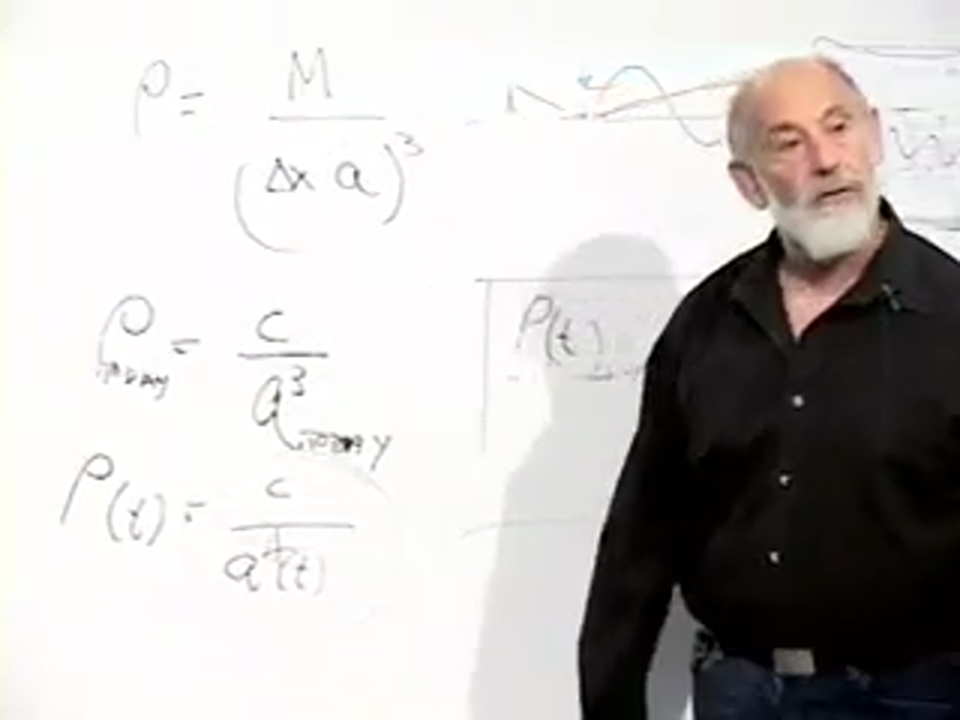
\includegraphics[width=0.72\textwidth]{lecture_09_figure_15.png}
  \caption{黑板上将物质密度关系推广到辐射标度 \(\rho_{\mathrm r}\propto a^{-4}\)。源帧在 01:29:20。}
  \label{fig:l09-radiation-board}
\end{figure}

在平坦弗里德曼方程中使用 \(\rho_{\mathrm r}\propto a^{-4}\) 得到
\begin{equation}
  \left(\frac{\dot a}{a}\right)^2=\frac{C_{\mathrm r}}{a^4},
  \qquad
  \dot a\propto a^{-1},
\end{equation}
因而
\begin{equation}
  \boxed{a(t)\propto t^{1/2}}.
  \label{eq:l09-radiation-solution}
\end{equation}
这比 \(t^{2/3}\) 增长得更慢。回溯到足够远的过去，辐射必定支配普通物质，因为当 \(a\) 减小时，\(a^{-4}\) 比 \(a^{-3}\) 上升得更快。讲座将物质-辐射交叉点置于尺度因子大约比今天小一千倍的时代附近。在该交叉点之前，宇宙由辐射支配；之后，在很长一段时期内，它由物质支配。

\section{真空能与指数膨胀}

真空能具有相反的标度行为。其密度是空无一物的空间的一种属性，并不随宇宙膨胀而稀释：
\begin{equation}
  \rho_\Lambda=\text{constant}.
  \label{eq:l09-vacuum-density}
\end{equation}
普通物质和辐射越回溯过去越致密，而这一项则不然。因此它在早期宇宙中较不重要，而随着其他组分稀释，它变得越来越重要。讲座使用当时的估计：真空能提供了今天宇宙能量密度的大约 \(70\%\)。

在\(\rho_\Lambda\)恒定的情况下，方程\eqref{eq:l09-flat-friedmann}给出恒定的膨胀率
\begin{equation}
  H_\Lambda=\sqrt{\frac{8\pi G}{3}\rho_\Lambda},
  \qquad
  \frac{\dot a}{a}=H_\Lambda.
\end{equation}
因此
\begin{equation}
  \boxed{a(t)=a(t_i)e^{H_\Lambda(t-t_i)}}.
  \label{eq:l09-vacuum-solution}
\end{equation}

\begin{figure}[H]
  \centering
  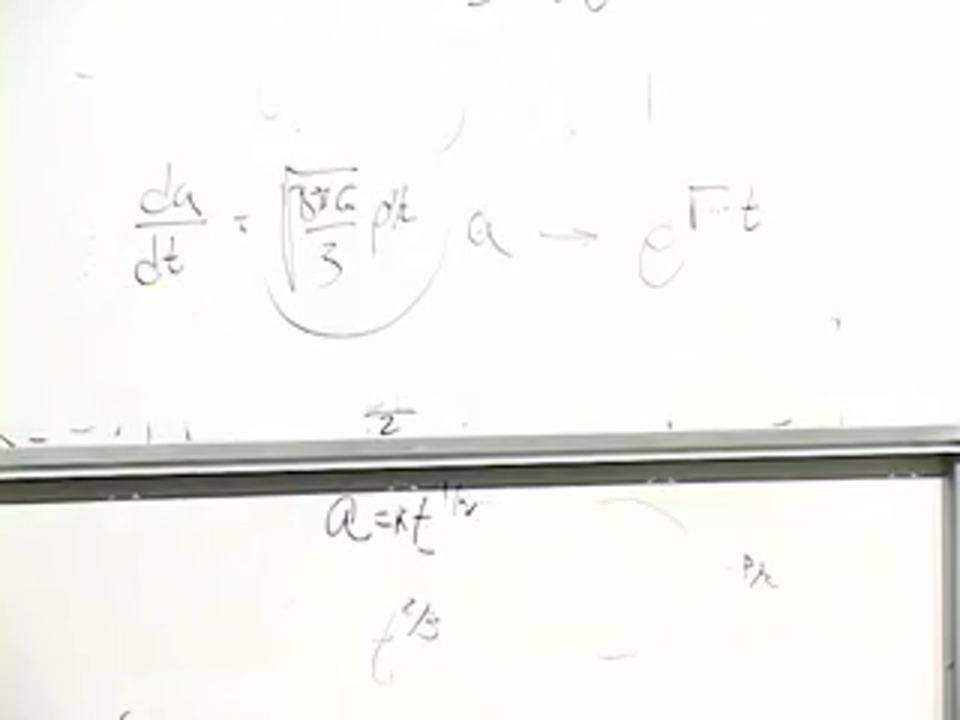
\includegraphics[width=0.72\textwidth]{lecture_09_figure_16.png}
  \caption{导致指数膨胀的常密度方程。
  源帧位于01:35:48。}
  \label{fig:l09-vacuum-board}
\end{figure}

在讲座中引用的观测尺度上，宇宙的线尺度在大约一百亿到一百二十亿年间翻倍。这一微小但非零的真空密度的起源仍未得到解释；它的存在及其对膨胀的影响是经验事实。

\begin{classroomqa}
\audiencequestion{在这一讨论中，真空能量与暗能量是同一回事吗？}
\lecturerresponse{是的。这里“暗能量”指恒定的真空能量密度，等价于宇宙学常数。可以设想更一般的随时间变化的暗能量模型，但它们不属于本讲座计算的一部分。}
\end{classroomqa}

\section{膨胀的宇宙如何使光红移}

\begin{classroomqa}
\audiencequestion{光子如何知道我们选择了膨胀的共动坐标，从而降低它们的能量？}
\lecturerresponse{它们并不对我们的标记作出响应。它们传播所经过的几何，其物理间隔在变化。占据一个物理尺寸翻倍的区域的波列，其波长也翻倍。共动坐标只是经济地描述这种拉伸；它们并不导致这种拉伸。}
\end{classroomqa}

\begin{classroomqa}
\audiencequestion{今天到达我们的背景光子来自哪里？}
\lecturerresponse{看得越远意味着看得越早。最终我们看到宇宙物质是电离等离子体的时代，由于光子被自由带电粒子反复散射，该等离子体是不透明的。光子能够最后一次自由地旅行到我们的那个边界，表现为围绕观测者的一个球面：最后散射面。}
\end{classroomqa}

\begin{figure}[H]
  \centering
  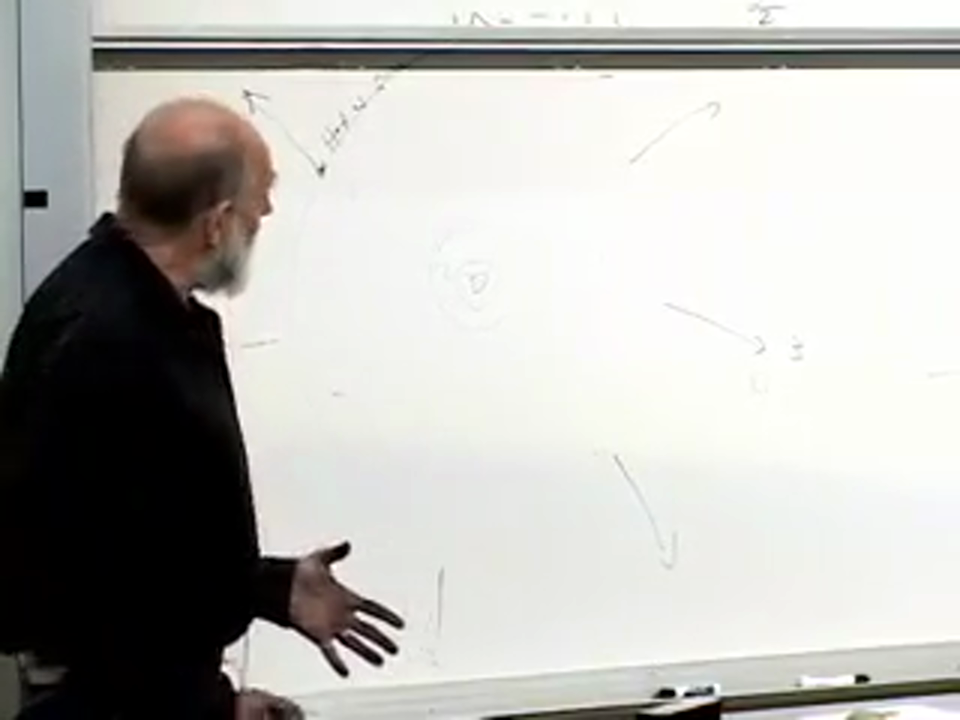
\includegraphics[width=0.72\textwidth]{lecture_09_figure_17.png}
  \caption{以观测者为中心的最后散射面及越来越远的壳层示意图。源帧位于01:42:05。}
  \label{fig:l09-last-scattering-board}
\end{figure}

\begin{figure}[H]
  \centering
  \begin{tikzpicture}[scale=0.9,>=Latex]
    \fill (0,0) circle (2pt) node[below] {observer};
    \draw[thick,orange!70!black] (0,0) circle (2.55);
    \node[orange!70!black,align=center] at (0,3.05)
      {surface of last scattering};
    \foreach \a in {25,75,145,210,285,335}{
      \draw[->,blue!60!black] ({2.55*cos(\a)},{2.55*sin(\a)}) --
        ({1.7*cos(\a)},{1.7*sin(\a)});
    }
    \draw[decorate,decoration={snake,amplitude=1.5pt,segment length=7pt},
      red!65!black,thick,->] (-2.5,0) -- (-0.15,0);
    \node[red!65!black,below] at (-1.35,-0.15)
      {redshifted photon};
  \end{tikzpicture}
  \caption{最后散射图像的清晰重建。}
  \label{fig:l09-last-scattering-clean}
\end{figure}

该辐射发射时具有热等离子体特征的光谱，到达我们时波长大约长了一千倍。用讲座中的多普勒语言来说，遥远的发射面迅速退行，其辐射被强烈红移。用几何语言来说，波在传播过程中被拉伸。两种图像编码了同一关系，
\begin{equation}
  1+z=\frac{\lambda_0}{\lambda_{\mathrm{em}}}
      =\frac{a_0}{a_{\mathrm{em}}}.
  \label{eq:l09-cosmological-redshift}
\end{equation}
\editorialnote{方程\eqref{eq:l09-cosmological-redshift}是讲座中拉伸描述和多普勒描述的标准定量形式。}

在更早的观测时代，最后散射球在相应的图像中会更近，而观测到的背景光子红移会更小，因此能量更高。随着宇宙时间推进，从那个早期等离子体到达共动观测者的光子波长越来越长。

\section{红移光子的能量去了哪里？}

\begin{classroomqa}
\audiencequestion{一个光子以能量\(h\nu_{\mathrm{em}}\)发射，到达时红移，能量更少。那部分差值发生了什么？}
\lecturerresponse{牛顿推导最初是一个能量方程。其宇宙学形式将膨胀率与物质能量密度联系起来，因此物质能量和膨胀不能作为分别守恒的账目来处理。讲座将丢失的光子能量描述为进入膨胀的动能记账。一个充满辐射的活塞使这个类比变得具体：辐射压将活塞向外推，光子波长增加，它们丢失的能量变成机械功和活塞的动能。}
\end{classroomqa}

\begin{figure}[H]
  \centering
  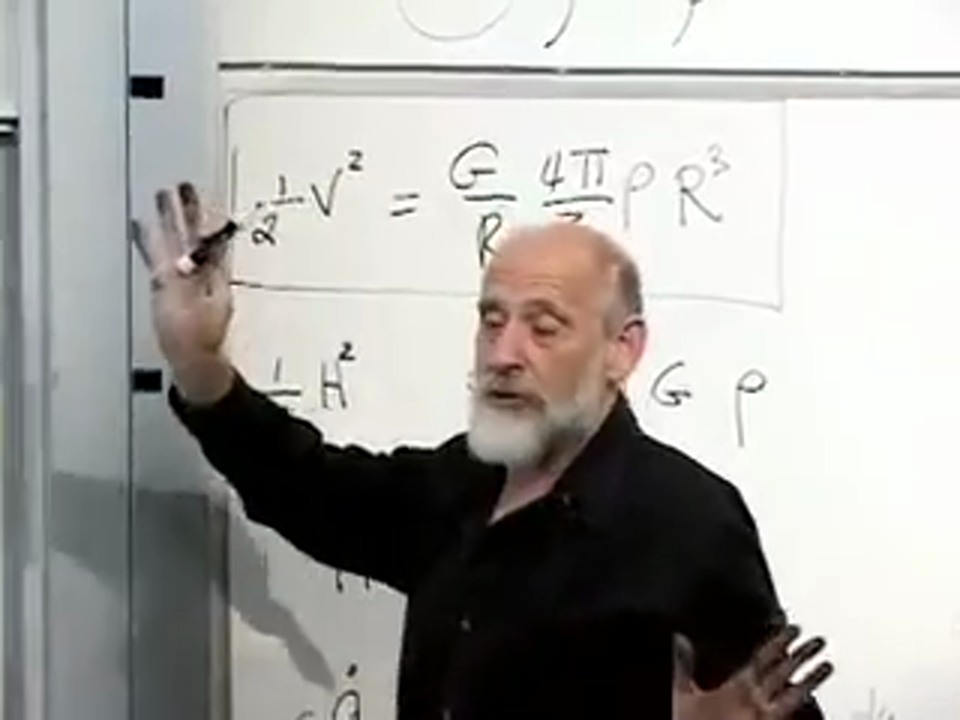
\includegraphics[width=0.72\textwidth]{lecture_09_figure_18.png}
  \caption{黑板上将方框中的牛顿能量方程置于相应的弗里德曼方程上方。源帧位于01:44:42。}
  \label{fig:l09-energy-bookkeeping-board}
\end{figure}

\begin{classroomqa}
\audiencequestion{是什么将辐射能量与膨胀耦合起来？}
\lecturerresponse{压强。在带有可移动活塞的圆柱体中，光子将动量传递给壁。当活塞移动时，辐射做功；其波长增大，能量下降。均匀膨胀的宇宙没有字面意义上的外部活塞，但\(p\,dV\)类比解释了为什么辐射的能量密度下降得比仅由数目稀释所导致的更快。}
\end{classroomqa}

\begin{figure}[H]
  \centering
  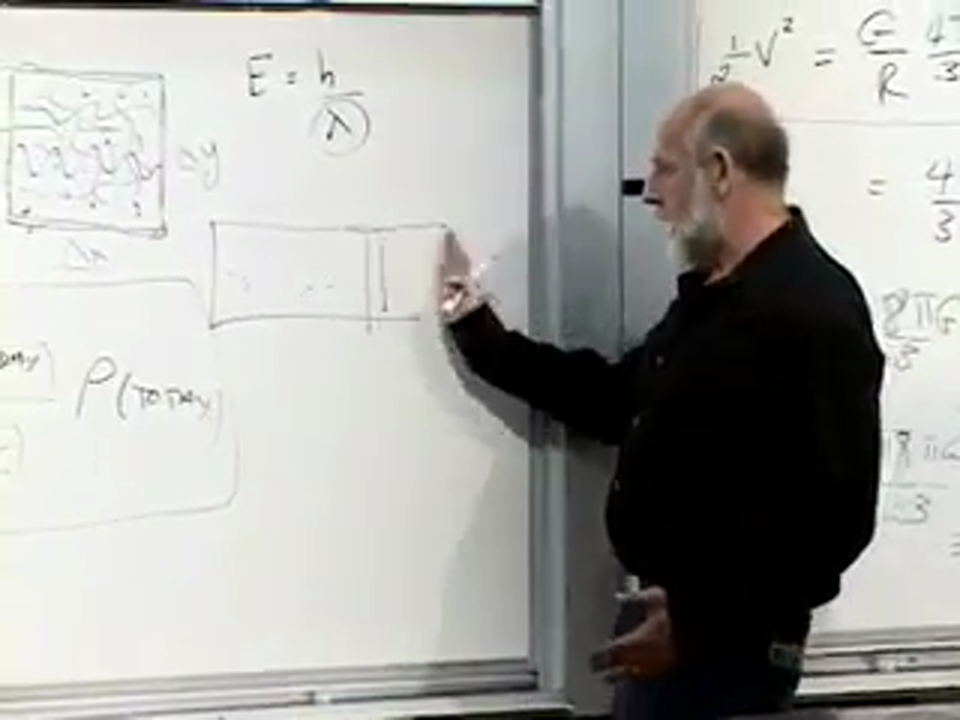
\includegraphics[width=0.72\textwidth]{lecture_09_figure_19.png}
  \caption{用于可视化压强做功的可移动充有光子的活塞。源帧位于01:46:40。}
  \label{fig:l09-piston-board}
\end{figure}

\begin{figure}[H]
  \centering
  \begin{tikzpicture}[scale=0.92,>=Latex]
    \draw[thick] (0,0) rectangle (5.3,2.6);
    \draw[very thick] (4.25,0) -- (4.25,2.6);
    \draw[very thick] (4.25,1.3) -- (5.25,1.3);
    \draw[->,thick,red!65!black] (5.25,1.3) -- (6.2,1.3)
      node[right] {moving piston};
    \foreach \y in {0.55,1.3,2.05}{
      \draw[decorate,decoration={snake,amplitude=1.4pt,segment length=6pt},
        blue!65!black,->] (0.35,\y) -- (3.9,\y);
    }
    \node at (2.15,-0.45) {radiation does \(p\,dV\) work};
  \end{tikzpicture}
  \caption{辐射-活塞类比的清晰重构。}
  \label{fig:l09-piston-clean}
\end{figure}

广义相对论中的能量需要谨慎处理。在一般的膨胀时空中，未必存在一个唯一的守恒全局能量，类似于孤立牛顿系统的能量。局域应力-能量守恒仍然成立，而对于均匀流体，它给出连续性方程
\begin{equation}
  \dot\rho+3H(\rho+p)=0,
  \label{eq:l09-continuity}
\end{equation}
其中包含压强做功项，正是物质与辐射标度律背后的原因。\editorialnote{方程 \eqref{eq:l09-continuity} 是讲座中刻意采用牛顿式能量记账类比所依据的精确局域广义相对论表述。}

真空能使得这一疑难尤为尖锐。由于其密度保持恒定而体积增大，共动区域内的总真空能增加。其负压强是引力源的一部分，并驱动加速膨胀。因此，不应要求朴素的“共动盒中的物质能量”单独守恒，而不把几何与压强做功包括在内。

\section{为什么标度因子可以从时间项中移除}

\begin{classroomqa}
\audiencequestion{为什么标度因子乘在度规的空间部分上，而不乘在时间部分上？}
\lecturerresponse{这是时间坐标的一种选择。假设从共形时间坐标 \(t\) 出发，有
\begin{equation}
  d\tau^2=A^2(t)\left(dt^2-dx^2\right).
\end{equation}
通过下式定义新的宇宙时间 \(T\)：
\begin{equation}
  dT=A(t)\,dt.
\end{equation}
于是
\begin{equation}
  d\tau^2=dT^2-A^2\bigl(t(T)\bigr)dx^2.
\end{equation}
时间微分前的公共因子已经消失，而物理标度因子仍留在空间项中。}
\end{classroomqa}

\begin{figure}[H]
  \centering
  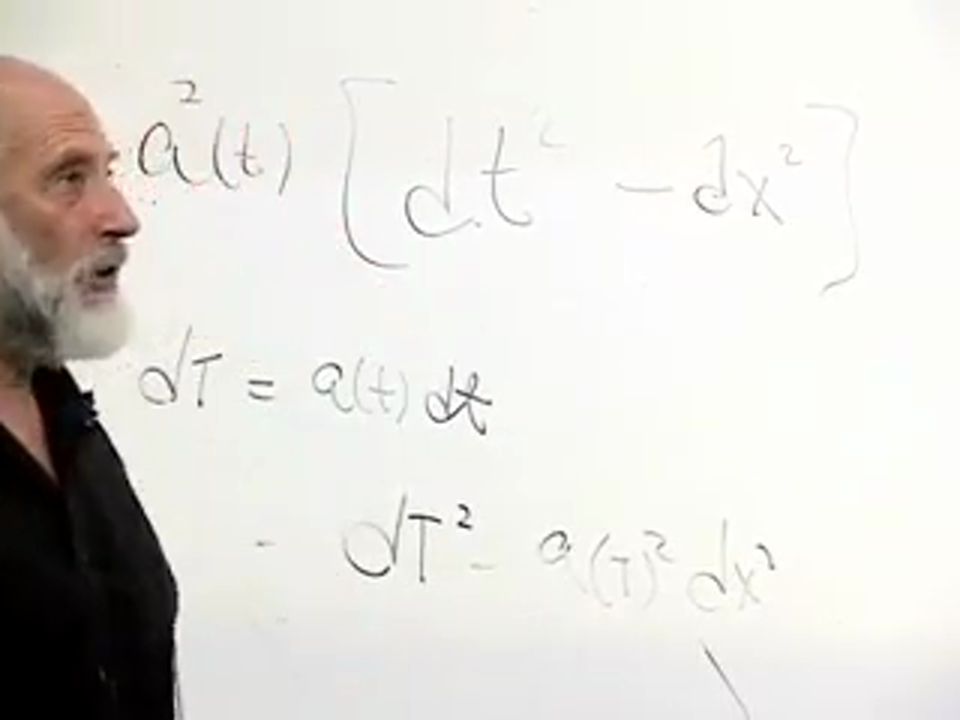
\includegraphics[width=0.72\textwidth]{lecture_09_figure_20.png}
  \caption{将共形时间转换为宇宙时间的时间重定义 \(dT=A(t)dt\)。源帧在 01：51：05。}
  \label{fig:l09-time-reparam-board}
\end{figure}

\section{曲率、真空能与宇宙命运}

\begin{classroomqa}
\audiencequestion{如果宇宙是正曲率的，我们是否应该已经看到星系朝我们运动而来？}
\lecturerresponse{未必。一个以低于逃逸速度发射的抛射体先向外运动，到达一个转折点，之后才落回。我们是在宇宙的膨胀阶段观测它。如果没有真空能，一个正曲率的物质宇宙最终会再坍缩。足够大的正真空能会阻止这一转折，而观测值似乎大到足以使长期膨胀呈指数式，无论空间曲率有多小。}
\end{classroomqa}

指数式的未来并非能量天堂。恒星最终会燃尽，物质与辐射密度呈指数式下降，遥远区域将超出因果接触。真空能仍然存在，而普通结构则变得越来越冷、越来越稀薄。

\begin{classroomqa}
\audiencequestion{向更遥远的过去看，光子是否比普通粒子更多？}
\lecturerresponse{光子与重子的数密度之比已经极其巨大，按讲座中的估计约为每个重子 \(10^{10}\) 个光子，而共动体积中的这两个数目都近似保持不变。向过去回溯时改变的主要是每个光子的能量。光子能量按 \(a^{-1}\) 上升，而非相对论性静止质量则不然。因此，尽管数目比本身未必改变，辐射在早期仍主导能量密度。}
\end{classroomqa}

核心教训是，仅凭几何并不能决定宇宙的历史。平坦的弗里德曼方程给出了膨胀与能量密度之间的关系，但物质内容提供了时间依赖关系。非相对论性物质给出 \(a\propto t^{2/3}\)，辐射给出 \(a\propto t^{1/2}\)，而恒定的真空能给出指数式膨胀。这三条定律组织了宇宙相继的各个时代，并解释了为什么同一个标度因子控制着距离、红移以及不断变化的哈勃参数。
